\chapter{数学知识表征}

知识的表征:人在自己的工作记忆和长时记忆中对信息表示形式,包括知识的\textbf{内化}、知识的\textbf{贮存}和知识的\textbf{再现方式}

\section{广义知识分类}

\[
\text{知识}
\begin{cases}
    \text{陈述性知识} \\
    \text{程序性知识}
    \begin{cases}
        \text{智慧技能} \\ 
        \text{认知策略}
    \end{cases}
\end{cases}
\]

\subsection{陈述性知识}

\textbf{定义}:关于事实或事物状况的知识,即描述“是什么”的知识。

\textbf{示例}:数学概念、命题,如“三角形外角等于不相邻两个内角之和”等。

\textbf{陈述性知识的获取:}
\begin{itemize}
    \item 新信息进入短时记忆,短时记忆中被激活的相关知识建立联系,而产生新的意义的建构。
    \item 采用复述策略、精致化和组织策略保持新建构的观念。
    \item 形成图式,并能将知识提取知识和运用于问题解决中。
\end{itemize}




\subsection{程序性知识}

\textbf{定义}:关于如何完成一件事情的知识,即由程序、步骤及策略组成的知识,描述“怎么做”的知识。

可以进一步分为两种亚类:
\begin{itemize}
    \item 智慧技能:用于相对自动化的情况,少受意识控制。强调高阶思维能力的运用和综合性。
    \item 认知策略:运用时较难达到自动化。强调个体如何调控和改进学习或思维过程。
\end{itemize}

\textbf{程序性知识的获取:}
\begin{itemize}
    \item 智慧技能(自动化技能):认知阶段、联系阶段、自动化阶段。
    \item 认知策略(策略性知识):受原有知识背景、反省认知水平、动机水平等多种因素影响。
\end{itemize}


\subsection{联系与区别}

\subsubsection*{联系}

\begin{itemize}
    \item 基础关系:陈述性知识是程序性知识的基础,程序性知识由陈述性知识转化而来。
    \item 核心成分:概念和规则既是陈述性知识的核心成分,也是程序性知识的核心成分。
    \item 表现形式:两类知识没有严格的分界,陈述性知识在被应用和转化后可以成为程序性知识。
\end{itemize}

\subsubsection*{区别}

1. 测量方式
\begin{itemize}
    \item 陈述性知识:可通过学习者的“陈述”方式测量。
    \item 程序性知识:能通过观察人的行为间接测量。
\end{itemize}

2. 心理表征
\begin{itemize}
    \item 陈述性知识:以图式表征。
    \item 程序性知识:以产生式系统表征。
\end{itemize}

3. 激活与提取
\begin{itemize}
    \item 陈述性知识:激活速度慢,提取过程相对静态。
    \item 程序性知识:激活速度快,提取过程是一个有意识的搜索过程,且能相互激活。
\end{itemize}

4. 输入与输出
\begin{itemize}
    \item 陈述性知识:相对静态。
    \item 程序性知识:相对动态。
\end{itemize}

5. 学习与遗忘速度
\begin{itemize}
    \item 陈述性知识:获得速度慢,遗忘也慢。
    \item 程序性知识:获得速度快,遗忘也快。
\end{itemize}

\subsection{数学过程性知识}

伴随数学活动过程的体验性知识

\begin{itemize}
    \item 一阶段:对知识\textcolor{red}{产生}的体验。体会知识产生的缘由,明晰新旧知识之间的关联和因果关系。
    \item 二阶段:对知识\textcolor{red}{发展}的体验。体悟知识发展的动因,包括数学学科的内部因素和促进知识发展的外部因素,习得探究数学问题的方法(逻相的和非逻辑的)和策略。
    \item 三阶段:对知识\textcolor{red}{结果}的体验。领会蕴涵在知识中的数学思想方法,感受数学结构的美。
    \item 四阶段:对知识\textcolor{red}{应用}的体验,体会数学应用的广泛性,积累解决问题的认知策略和元认知知识,形成自我监控的意识和习惯。
\end{itemize}


\section{陈述性知识表征}

\[
\text{图式}
\begin{cases}
    \text{网络命题表征} \\
    \text{表象表征} \\
    \text{线性排序}
\end{cases}
\]

\subsection{网络命题表征}

\subsubsection*{基本单位——命题}

\textbf{命题}——由一种\textbf{关系}和一组\textbf{论题}构成

\textbf{关系}——由动词、副词、形容词、介词等表达

\textbf{论题}——指概念,由名词或代词表达

\textbf{命题网络}——通过\textbf{共同成分}将多个命题联系起来


\begin{multicols}{2}

\subsubsection*{模型1——层次网络模型}

按概念的从属关系相应地实行分级贮存

在每一级概念的水平上,只贮存该级独有的特征

同一级的各概念所具有的共同特征贮存于上一级概念的水平上

\textbf{缺陷}:忽视了各层次概念之间和同一层次概念之间的横向联系

\columnbreak

\subsubsection*{模型2——激活扩散模型}

用结点\textbf{表示概念}

以语义联系或语义相似性来\textbf{组织概念}

以联线表示概念间的联系,联线长度\textbf{表示联系的紧密程度}

\end{multicols}


\subsection{表象表征}

概念——人们借助于事物知觉的表象去记忆或贮存陈述性知识的方式

特征1——能对事物在各个方面的一些物理特征作出连续保留

特征2——是数学学习中知识表征的重要形式(同一个概念既有代数意义,又有几何意义)

\subsection{线性排序}

概念——人们利用事物间的顺序来表征事物

例1——A>B, B>C, A<D, C<E, B>E

\begin{itemize}
    \item 与命题的区别:命题仅保留了其中所提及的论题间的关系,而不涉及这些论题次序作出排定。
    \item 与表象的区别:表象保留知觉结构之间的间隔关系,线性排序则是对一组元素的顺序作了排列,但不涉及各元素之间的距离。
\end{itemize}

\subsection{图示}

概念——对陈述性知识的综合表示,是三种表征的整合

\begin{figure}[htbp]
    \centering
    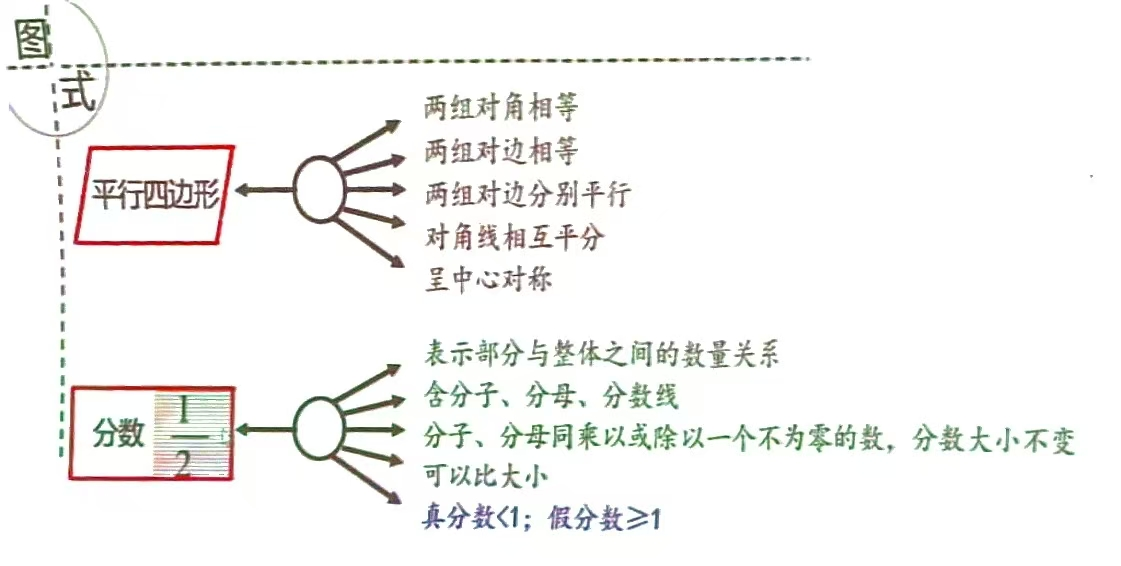
\includegraphics[width=0.5\linewidth]{image/tushilizi.jpg}
\end{figure}

\subsection{数学陈述性知识的表征补充}

图示(命题网络、\textcolor{red}{表象}、线性排序)

数学概念的表象:

\noindent
对事物在知觉基础上所形成的感性形象

\noindent
想象表象——个人通过自己的想象去构造一种可以表述对象的模型

例如,对于集合语言“A是8的真子集”,可以想象为“圆A位于圆B之中”。

\noindent
实例表象——将一个抽象的、一般的数学对象用其特例来进行表征

例如,从数转化到字母符号,数即为字母的特例,学生学习字母之间的有关运算时,往往把它和数对应起来,表征为数的运算,这就是一种实例表征。

\section{程序性知识表征}

\subsection{产生式}

概念——一条“如果……那么……”规则

换言之——对某一或某些特定条件满足时才发生某种行为所编的程序

产生式系统——一系列重叠产生式

\subsection{数学程序性知识的表征补充}

\begin{itemize}
    \item 数学程序性知识的表征是一种双向产生式。
    \begin{itemize}
        \item 既指令“什么条件下会有什么动作”,又指令“不同情形中选用不同的产生式”
    \end{itemize}
    \item 数学程序性知识表征产生式中的条件或结论可能不是唯一的。
    \item 数学程序性知识的产生式往往是一个重叠的系统。
\end{itemize}


\section{数学过程性知识的表征}

\begin{itemize}
    \item 关系表征——个体对知识发展过程中知识之间存在某些关系的体悟。
    \begin{itemize}
        \item 具体地说,它相当于陈述性知识的命题网络中连结命题的连线,以及程序性知识的产生式系统中连结产生式的连线。
    \end{itemize}
    \item 观念表征--对知识之间发生关系的缘由的体悟。
    \begin{itemize}
        \item 其成分更多是一种\textbf{元认知体验}。
    \end{itemize}
\end{itemize}




\begin{problemset}[习题]
  \item 知识以何种方式贮存在头脑中?
  \item 举例说明什么是表象表征?
  \item 举例说明什么是线性排序表征?
  \item 陈述性知识与程序性知识的联系与区别
  \item 图式、命题表征、线性排序、表象、产生式之间的联系与区别
  \item 陈述性知识、程序性知识、过程性知识的联系与区别
  \item 命题网络表征中知识是以何种关系贮存在一起的?
\end{problemset}
